\chapter{How do you learn? A survey to lifelong learners on mobile usage habits}

\vfill
This chapter presents the results from a questionnaire filled out by 147 lifelong learners with the aim to analyse learning practices of adults, and to recognise patterns of lifelong learners in order to support them with technology. These patterns capture the context in which lifelong learners learn, i.e. the day of the week, duration, location activity being performed, type of device being used, way to interact with their devices and how these aspects can affect when an adult student takes the initiative to learn. As an outcome of this work, important research questions to provide technological support for lifelong learners in daily physical spaces are raised.
\vspace{3em}

This chapter is published as: 

Tabuenca, B., Ternier, S., \& Specht, M. (2013). Supporting lifelong learners to build personal learning ecologies in daily physical spaces. \em International Journal of Mobile Learning and Organisation\em, 7(3), 177-196.

and

Tabuenca, B., Ternier, S., \& Specht, M. (2012). Everyday patterns in lifelong learners to build personal learning ecologies. In M. Specht, J. Multisilta, \& M. Sharples (Eds.), \em Proceedings of the 11th World Conference on Mobile and Contextual Learning\em (pp. 86-93). October, 16-18, 2012, Helsinki, Finland.
\clearpage

\section{Introduction}
Lifelong learners are confronted with a broad range of activities they have to manage every day. In most cases they have to combine learning, working and everyday life throughout the day. For the support of lifelong learners, their daily practices and learning patterns are of importance. Lifelong learning includes a variety of different educational scenarios and contexts in which learners operate. These contexts include traditional formal programmes, non-formal education, on the job-training, and informal learning. \cite{Fischer} even values lifelong learning as a mindset that people have to acquire including the following learning scenarios: self-directed learning, learning on demand, collaborative learning and organisational learning.

One of the most critical challenges for the implementation of lifelong learning is to integrate real world problems and learning in the same process. One promising approach to connect the world of working and learning is a pattern approach. According to \cite{Alexander1977} each pattern describes a \em�problem, which occurs over and over again in our environment, and then describes the core of the solution to that problem�\em. \cite{Rohse2006} propose design patterns that should enable the detailed formalised description of \em�the dynamics between learning and technologies without the potential ideological or pedagogical mask of teaching in formal education and training settings�\em. In the setting of an adult lifelong learner, this is especially difficult as in most cases interests might be highly distributed over different domains and keeping up learning needs an extra effort. Lowing the barriers for access to relevant information and support services anywhere, anytime, and anyhow is one essential component for efficient lifelong learning support.

The idea of a Personal Learning Environment (PLE) recognises that learning is ongoing and seeks to provide tools to support this kind of learning. It also recognises the importance of the individual to organise his or her own learning in order to embed it in contexts of daily life \citep{Attwell2007a}. Personal learning has been hierarchised into learning activities, episodes and projects \citep{Vavoula2002,tough1979adult}. \cite{Vavoula2002} define learning activity as the distinct acts that the person carries out during reading, discussing, listening and making notes. \cite{tough1979adult} defines a learning episode as a well-defined period of time that is held together by the similarity in intent, activity or place of the thoughts and actions that occur during it; it has a definite beginning and ending in time. Learning projects are formed by grouping episodes together on the basis of their contingency in terms of purposes and outcomes that could happen at different locations.

Smartphones have been pinpointed as a key learning partner, not only because of their affordances supporting learning activities (camera, bigger screens, location capabilities, audio and video player and recorder, sensors etc.), but also because they provide utilities to track users lifelong learning. There are everyday scenarios built by lifelong learners in recognition of the places where they perform interactions with spaces, artefacts and resources through which people achieve their work. \cite{Wong2012} advocates the combination of a cloud-based learning hub account, a smartphone, and additional notebook/desktop computers as an ideal technical setting for a personalised seamless learning environment.

This chapter analyses the results of a questionnaire for lifelong learners classifying the results according to the following criteria: type of mobile device; lifelong learners behaviour, timing, motivation, physical spaces where learning takes place, learning activity being performed, and gender.
\section{A questionnaire on mobile usage habits}
\subsection{Method}
This survey was completed by 147 lifelong learners (See demographics in table \ref{tbl:chap1table1}). The questionnaire was distributed both in English and Spanish taking advantage of the following channels: social networks, three Dutch and Spanish universities, two high schools from Belgium and The Netherlands, two companies, one academy for skills-training and the authors blog. The survey was stored in an online platform so that everybody could access and fill out the questionnaire making use of the distributed URL. Answers were collected over the course of three months. Participation was voluntary and unrewarded.

The questionnaire is composed of 21 items \citep{Tabuenca2012}(Appendix A): five multiple choice questions, six single select questions, nine matrix selection questions, and one open answer question. An introduction section (60 words) was included in order to explain the aim of the questionnaire and to define frequently used concepts within the items. These concepts are: \em(a) mobile device: regular phone, smartphone, tablet, multimedia player and laptop when used not always in the same place; (b) learn: taking the initiative to learn something actively. It can be related to work, current studies or self-fulfilment\em.

There are four questions about demographics (age, gender, occupation, and professional domain), three questions about usage patterns with mobile devices, two questions about how timing and content are related, seven questions linking activities, locations, and ways of interaction with lifelong learners mobile devices, one question identifying difficulties when learning with mobile devices, three questions about the lifelong learners motivation, and one more question to estimate how familiar is the concept of \em lifelong learning \em for the participants.

The data with the answers have been exported from the online survey platform to a spreadsheet file. This file has been imported with a database engine in order to create a table for each of the questions in the survey. A database client has been used to build joining-table queries, aiming to find patterns in the answers given in different questions. Chart reports have been created from these requests to carry out the analysis.

The results of this questionnaire are presented including references to previous studies on mobile device usage patterns and mobile learning support, in order to contrast and corroborate the conclusions.
\begin{table}[h]
  \small
  \centering
  \caption{Survey on mobile usage for learning. Demographics}
  \label{tbl:chap1table1}
\begin{tabular}{llcc}
\thickhline
\textbf{Variables}  & \textbf{Levels}   & \textbf{\begin{tabular}[c]{@{}c@{}}Number\\ of subjects\end{tabular}} & \textbf{\begin{tabular}[c]{@{}c@{}}Percentage \\ of subjects\end{tabular}} \\ \thickhline
Gender              & Male              & 86                                                                    & 59                                                                         \\ 
                    & Female            & 61                                                                    & 41                                                                         \\ \hline
Age                 & Under 25          & 43                                                                    & 29                                                                         \\ 
                    & 25-34             & 50                                                                    & 34                                                                         \\ 
                    & 35-44             & 27                                                                    & 18                                                                         \\ 
                    & 45-54             & 14                                                                    & 10                                                                         \\ 
                    & 55-65             & 13                                                                    & 9                                                                          \\ 
                    & Older than 65     & 0                                                                     & 0                                                                          \\ 
Professional domain & Computer sciences & 41                                                                    & 27                                                                         \\ \hline
                    & Engineering       & 24                                                                    & 16                                                                         \\ 
                    & Natural sciences  & 16                                                                    & 10                                                                         \\ 
                    & Humanities        & 16                                                                    & 10                                                                         \\ 
                    & Business          & 13                                                                    & 9                                                                          \\ 
                    & Law               & 8                                                                     & 15                                                                         \\ 
                    & Medicine          & 3                                                                     & 2                                                                          \\ 
                    & Other             & 34                                                                    & 21                                                                         \\ \hline
Professional status & Employed          & 99                                                                    & 67                                                                         \\ 
                    & Student           & 48                                                                    & 33                                                                         \\ 
                    & Self-employed     & 11                                                                    & 7                                                                          \\ 
                    & Homemaker         & 3                                                                     & 2                                                                          \\ 
                    & Unable to work    & 1                                                                     & 1                                                                          \\ 
                    & Retired           & 0                                                                     & 0                                                                          \\ \hline
\end{tabular}
\end{table}
\subsection{Results}
\subsubsection{What is 'lifelong learning'}
Participants were given the following definition of lifelong learning: \em�All learning activity undertaken throughout life, with the aim of improving knowledge, skills and competences within a personal, civic, social and/or employment-related perspective� \em (European Commission, 2011). When participants were asked whether they considered lifelong learners themselves, 21.76\% reported a negative answer. However, paradoxically the same respondents answered positively to the question \em Do you have a natural motivation to learn? \em

\subsubsection{Patterns based on the type of device, user's behaviour and timing}
The presence of mobile devices in lifelong learners' daily activities is a fact that can be gathered from the results of this questionnaire. Portable computers are used every day by 70.06\% of the respondents. Smartphones are used every day by 56.46\% of the respondents, while 17.68\% use their tablet on a daily basis.

Trends indicate that smartphones and tablets are the cornerstone in future learning designs since they are even more portable than portable computers. The smartphone is easily carried around in a pocket and can be used in any moment of the day. A study performed by \cite{Arbitron2011} concluded that engagement with different smartphone features is divided evenly during the day, detecting a slight peak in the afternoon from 15h to 18h.

Our results show that there are two time slots of the day in which lifelong learners feel more motivated to learn, these are from 10 h to 12 h (55.78\%) and from 16 h to 20 h (49,66\%). This discontinuity is happening due to the pause to have lunch, in which generally people change their context, commute or change their location for some time. Our study (see Figure \ref{survey_fig:2}) shows a difference for perceived motivation to learn between people that own a smartphone and those that do not own one. Individuals that own smartphone expressed to be more constantly motivated during the day than non-smartphone users.
\begin{figure}
     \centering
     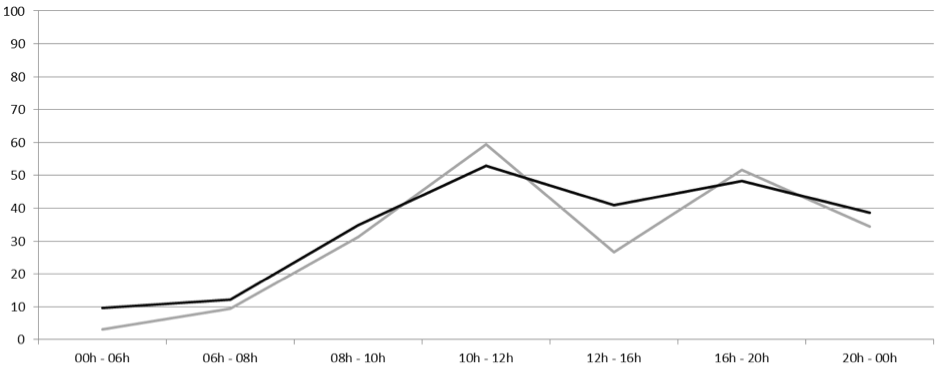
\includegraphics[width=0.9\linewidth]{img/survey_fig2}
     \caption{Motivation to learn during the day. Smartphone users (black line) vs non-smartphone users (grey line)}
     \label{survey_fig:2}
\end{figure}
A study by \cite{Eoff2011} based on one-week click data from Bitly (online link tracking platform) concluded that tablets (iPads) usage during the day is not flat and drastically different when compared to other types of devices, including smartphones and portable computers. Their results suggest that usage lowers after breakfast, remains low during traditional working hours and does not peak until much later in the evening (19 h�00 h). The results of the questionnaire for lifelong learners suggest that there is an association between tablet users and their motivation to learn. The percentage of tablet users motivated to learn was 10\% higher than with individuals that do not use tablets (see Figure \ref{survey_fig:3}). In relation to the peak observed late in the evening by \cite{Eoff2011}, our results show that the learning-motivation-curve in tablet users in the last hours of the day does not descend so much in comparison to non-tablet-users.
\begin{figure}
     \centering
     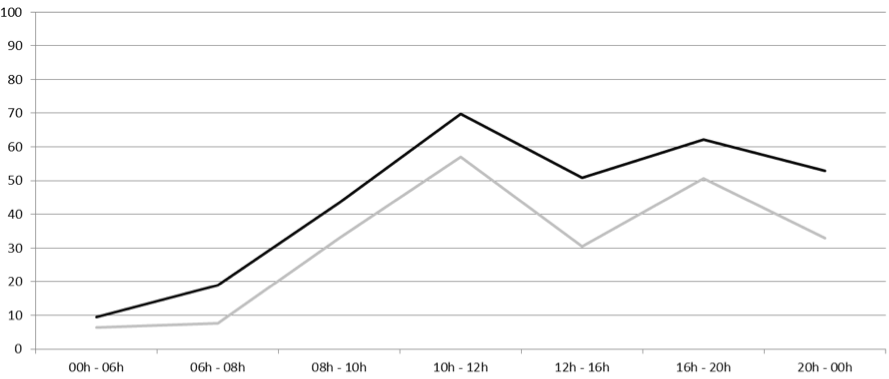
\includegraphics[width=0.9\linewidth]{img/survey_fig3}
     \caption{Motivation to learn during the day. Tablet users (black line) vs non-tablet users (grey line)}
     \label{survey_fig:3}
\end{figure}
\cite{Eoff2011} suggest that tablets are mainly used for entertainment purposes since they are less used than the rest during working times. Tablet usage is higher than the rest of the devices during leisure time. This effect can be also observed during the weekend when tablets usage between 8 h and 15 h is higher than during the week at those same hours. No other device sees a heavy increase of use during the weekend.

When asking lifelong learners on which days of the week do they spend more time with their mobile device(s), our results show (see Figure \ref{survey_fig4}) that the usage for smartphone users is flat with a slight peak on Friday as well as a higher percentage in contrast to non-smartphone users. There is an increase of 30\% in non-smartphone users from a working day (Thursday) to weekend day (Saturday).

There are different ways of consuming learning content on mobile devices: \em listening, reading, writing, watching\em, and \em gaming\em. When lifelong learners were asked how long on average they spend on each of these activities, 21\% of the individuals reported to listen more than one hour per day to their mobile devices. This preference for listening can also be inferred from the results in which 64.62\% of the respondents reported to use their media players at least once a week.

When lifelong learners were asked how much time do they spend on different topics per day, the outcome was that \em study\em, \em music \em and \em social networking \em are the activities on which they spend most of their time. In contrast to these results, the study performed by \cite{Arbitron2011} with similar topics indicates that messaging, browsing, social networking and voice are the activities on which individuals spend more time.

Examining the way in which individuals check their mobile phone for a new SMS, missed call, email or any other notification, there are two different behaviours that can be highlighted from the results of the questionnaire. There is a first group of individuals (37.41\%) that only check incoming notifications when the device notifies them with an alert. The second behaviour is performed by the individuals (34.68\%) that check it continuously (at least once per hour). Comparing behaviours between genders, it is remarkable that the option \em I only check my mobile when it alerts me \em was answered by 44\% of the men and 28\% of the women. Women's behaviour was more evenly distributed among the rest of the options (once a day and once every four hours).
\begin{figure}
     \centering
     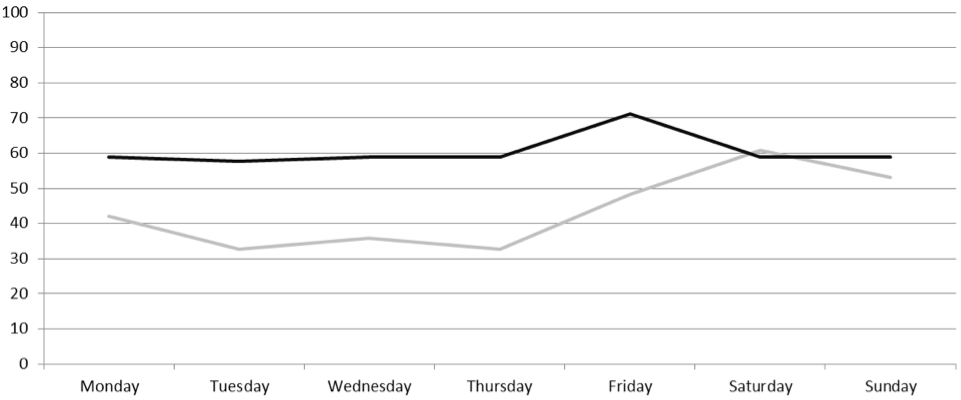
\includegraphics[width=0.9\linewidth]{img/survey_fig4}
     \caption{Mobile device(s) usage during the week. Smartphone users (black line) vs non-smartphone users (grey line)}
     \label{survey_fig4}
\end{figure}
\subsubsection{Linking locations, activities and ways of interaction with mobile devices}
A study performed by \cite{Google2011} on 5013 adults, concluded that there are two main situations where they use smartphone: 1) being at home (93\%); 2) on-the-go (87\%). Moreover, adults were asked for the most common context in which they use Internet on their smartphone. The highest rate was obtained (59\%) for the activity \em Waiting \em (in the line at the market, doctor, office, bus, etc.). This questionnaire has focused on three learning contexts (at home, on the move, and waiting times) including six items to identify patterns linking locations (living room, kitchen, bathroom, working/sleeping room, on-the-move and, waiting for someone), actions normally performed in those locations (e.g. having breakfast, brushing your teeth, lying on bed, etc.), and ways of interaction with mobile devices (listen, watch videos, write and read), also defined as \em learning activities \em by \cite{tough1979adult}. These results have raised some interesting differences regarding the way in which participants reported to behave depending on their gender.
\subsubsection{At home}
\em Sitting in the sofa \em is the most popular place to interact with mobile devices, not only compared to any activity performed in the living room or anywhere at home, but also outdoors and on-the-move. Exactly 62.58\% of respondents reported that they normally \em read \em contents, 50.34\% \em write \em contents, 44.89\% \em watch \em videos and 34.01\% \em listen \em to audios while being in the sofa. The \em living room \em was reported to be the most popular place to read contents, and specifying more, \em being sat in the sofa \em and \em watching TV during advertisement time \em (47.61\%). There was also a high rate of respondents that reported to write contents while \em watching \em TV during advertisement time (32.64\%).

One finding that can be gathered from responses regarding the context \em in the bathroom \em is that this intimate place has a significant association with mobile device interaction when used for listening. Individuals reported to listen while having a shower (23.12\%), making-up/shaving (18.36\%) and brushing their teeth (18.36\%). Being on the toilet is the most compatible activity with the different ways of interaction, i.e. 33.33\% of the respondents used their mobile device to \em read \em, 21.08\% to \em write \em and 11.56\% to \em listen \em. Similar, the poll performed by \cite{Google2011} stated that 39\% of the adults had used the Internet on their smartphone while \em using the bathroom \em, and 8\% while taking a \em shower/bathing \em.

The majority of the respondents (54.42\%) reported that they normally read contents on their mobile devices while \em being sat at the desk \em, 51.69\% \em read \em, 37.41\% \em listen \em and 29.92\% \em watch videos \em, this means that the \em desk \em is the best place to interact with mobile devices while \em being in the room \em. Furthermore, the \em bed \em is suited to interact with mobile devices \em reading\em (50.33), \em listening \em (34.69), \em watching \em (34.01\%) and \em writing \em (33.32\%).

The \em kitchen \em is a location associated with \em listening \em on mobile devices. The results from this questionnaire suggest the same effects than the ones observed to the context in the bathroom where mobile devices are mainly used for \em listening \em. The main contexts in which participants embed their listening-learning-activity are while \em cooking \em (30.6\%) and \em heating the breakfast \em (25.84\%). It is only remarkable that 16.32\% of the respondents interact with their mobile devices to read contents while \em cooking \em (probably requesting cook-recipes or short messaging while boiling, frying or anything in the oven). Similar, the survey by \cite{Google2011} indicated that 27\% of the participants had used the Internet on their smartphone while \em cooking/and or other household chores \em.
\subsubsection{Waiting times}
Rates varied from 15.64\% (being in the airport) to 4.76\% (waiting in a commercial centre). The \em bus \em stop (43.52\%) and the \em train station \em (41.49\%) seem to be the most suitable places to interact with mobile devices \em reading \em contents. When \em writing \em on mobile devices, the highest rates are evenly distributed (approximately 38\%) for the following contexts: \em waiting \em at the \em bus stop\em, at the \em train station \em and \em anywhere in the street \em. Results depict that waiting times are not normally used to consume video contents in contrast to the rest of the ways of interaction (listen, read, write). 
\subsubsection{On-the-move}
The results from the study performed by \cite{Kim2005} indicate that the most common context for using mobile Internet is described as follows: \em �participants have a hedonic goal, their emotional state is high, their legs are stopped, visual and auditory distractions were low� \em, few people are around them, and their interaction is low. This is a different picture from the widely held belief that the mobile Internet would be used often while moving outdoors. However, mobile devices have improved their capabilities to access the Internet, e.g. bigger displays, touch screens and faster connections and mobile interaction with smartphones is different nowadays. Our results suggest that interactions with mobile devices on-the-go are frequently carried out \em listening \em, being in the train 51.69\%, 50.33\% bus, and walking 48.3\%. \em Reading \em contents is the second most popular way of interaction when moving, 50.33\% by train, 40.82\% by bus, and 36.73\% accompanying the car driver. The train is the most popular place to interact with mobile devices while listening,\em reading \em and writing, whereas the plane is the most popular place to \em watch videos \em. Similar, the poll performed by \cite{Google2011} stated that 43\% of the individuals had used the Internet on their smartphone while commuting to work/school and 20\% driving by vehicle.
\begin{figure}
     \centering
     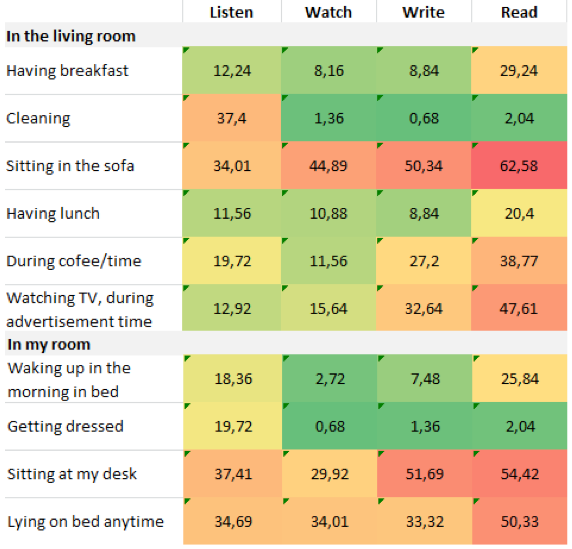
\includegraphics[width=0.8\linewidth]{img/survey_fig5}
     \caption{Learning activities in context with mobile devices. Percentage of individuals. The higher (red) the percentages the more popular the locations/activities are}
     \label{survey_fig:5}
\end{figure}
\subsubsection{Gender}
Regarding the gender effects, our results show some evidence on the fact that certain learning activities were more pronounced in men than women and vice versa (see Figure \ref{survey_fig:6}). On the one hand, there are a 44.18\% of men that reported to use their mobile devices \em reading \em contents while being sat on the toilet; however, only 18.02\% of the women do so. This difference was also notable for \em writing \em contents (29.05\% men vs. 9.83\% women) and \em watching \em videos (15.11\% men vs. 3.27\% women). However, gender did not moderate the effects of listening contents. On the other hand, differences were also found regarding \em listening \em to contents in some particular places. Women reported to be more willing to use their mobile devices while cooking (42.60\% women vs. 22.08\% men), sorting groceries (26.21\% women vs. 5.81\% men) in the kitchen, and cleaning in the living room (49.16\% women vs. 29.05\% men). Moreover, it is remarkable that for the context \em waiting \em in a commercial centre, 37.24\% of the men reported to read contents in their mobile devices while only 16.38\% of the women reported so.
\begin{figure}
     \centering
     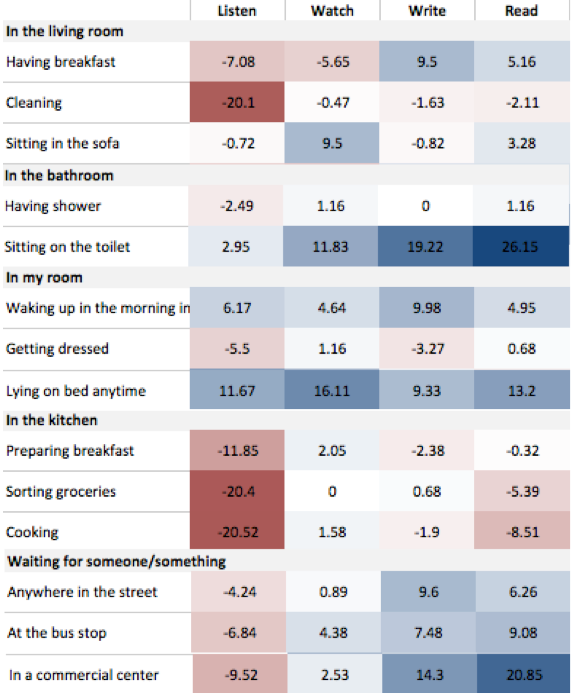
\includegraphics[width=0.8\linewidth]{img/survey_fig6}
     \caption{Learning activities in context with mobile devices. Difference in percentages between men and women. Positive (blue) numbers represent higher male percentage. Negative (red) numbers represent higher female percentage}
     \label{survey_fig:6}
\end{figure}
\subsubsection{More learning activities}
Participants were asked whether they had missed in the questionnaire any other activity where they usually get along some learning episode using their mobile devices. Some of them reported sport activities like running, cycling or at the gym, on-the-go activities like taking a walk or walking the dog, and some other miscellaneous ones like having lunch/dinner alone in a bar, feeding the infant, taking care of infant, and while doing some do-it-yourself labour at home (carpentry, plumbing...). Similar, the poll performed by \cite{Google2011} concluded that 48\% of the adults had been eating while using the Internet on their smartphone, 17\% walking their dog and 13\% playing sports. Another respondent reminded us that there are no patterns for every situation reporting \em I just learn something when I find the time \em.

\subsubsection{Difficulties learning with mobile devices}
\cite{Wong2011d} identified ten seams by which learning experiences are disrupted today and for which Mobile-assisted Seamless Learning (MSL) technology has to find new solutions. The identified ten gaps (MSL1-10) in seamless learning support are of high relevance for lifelong learners. Participants were asked about seven of these ten gaps in two items of the survey. The remaining three gaps (MSL5, 9, 10) were too complex concepts to deal in this poll and will be treated in suitable future studies.

In previous sections we have provide evidences to confirm the existence of barriers to learn: across location (MSL4) and across time (MSL3) gaps. Some cues are also exposed on how to cover these gaps supported with mobile technology. Participants were requested to report how often do they encounter these difficulties (MSL1-3 and MSL6-8) when learning and assisted with their mobile devices. The results from the questionnaire indicate that participants varying from 12\% to 17\% in the different MSLs usually find these difficulties. Nevertheless, approx. 34\% of the respondents reported not a difficulty in all these difficulties. The most reported difficulty was \em finding suitable slots of time during the day \em with a 21.08\% of the respondents that reported to have it usually and a 4.76\% that find it always. Slightly higher rates to the three resting difficulties, and with similar rates between them were the \em combined use of multiple device types (laptop, mobile phone and/or tablet) \em and the \em linking real world to what I learned digitally \em with approximately 17\% of the respondents that usually found these difficulties.

\section{Conclusions}
The aim of the questionnaire for lifelong learners is to analyse daily learning activities in adults to recognise patterns in lifelong learners and shed light on ways to support them with technology. The analysis of the results arises the ten following findings:

\begin{figure}
     \centering
     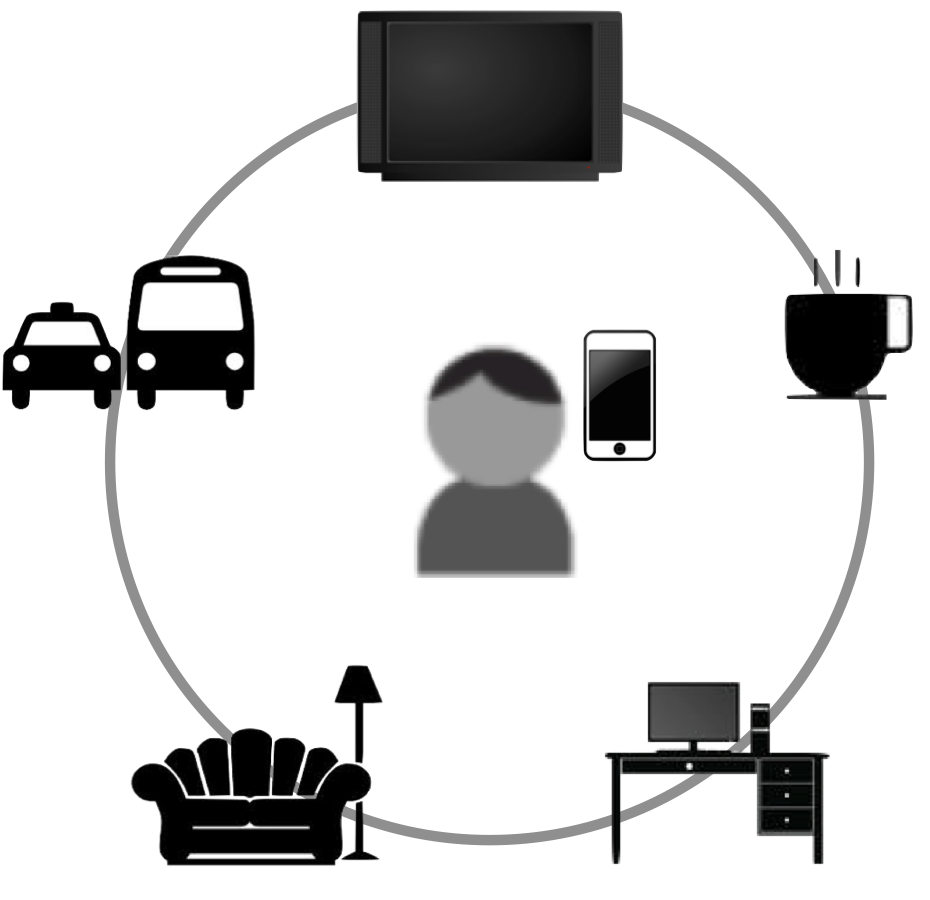
\includegraphics[width=0.5\linewidth]{img/survey_fig9}
     \caption{User's learning environments throughout the day}
     \label{survey_fig:6}
\end{figure}

\begin{enumerate}
\item Portable Computers are the most commonly used device for learning. Recent studies \citep{Wesel2011} have found similar results arguing ergonomic reasons. Students prefer bigger screen in contrast to smaller screens from smartphones or tablets.
\item Individuals that own a smartphone reported to be more constantly motivated to learn during the day than non-smartphone users.
\item Individuals that own a smartphone use it constantly during the whole week. The rest of the individuals reported lower usage during working days and an increase during the weekends.
\item \em Listening \em  is the most compatible learning activity when performing other tasks at the same time. It is also the one in which adults spend more time and in longer time slots. These results envision that audio contents are well suited for distributing learning materials as they can be consumed from most devices.
\item There are two different behaviours when adults check their mobile phone for a new SMS, missed call, email or any other notification. There is a group that only checks incoming notifications when the device notifes them with an alert. There is another group that check it continuously. These results suggest that these two behaviours must be taken into account when designing mobile applications for learning. 
\item There is an association between the learning activity being performed (\em reading, listening, writing or watching \em) and the concrete location where it takes place. Some patterns were found in the way to interact with mobile devices while being at home and depending on the room where the individuals were located. Participants were more willing to perform any kind of activity with their mobile device(s) while being in the living room or in the sleeping/working room. Nevertheless, participants reported that the kitchen and the bathroom were places where they use to perform the \em listening \em learning activity.
\item Learning activities are mainly performed when adults are with their legs stopped. The \em reading\em and \em writing \em learning activities mostly take place being sat (sofa, desk, train, bus and toilet) or lying on somewhere (bed). Sitting in the sofa is the place where adults reported the higher acceptance when carrying out any learning activity. However, the listening learning activity that takes part more evenly in the different locations and embedded in different activities.
\item Men and women behave different when making use of their mobile devices. These results suggest that men and women seem to behave differently in the way they perform learning activities as well as the way to dispatch incoming notification on their mobile phones. Furthermore, the study performed by \cite{Ofcom2010} stated that men spend nearly an hour more per day using media than women.
\item Lifelong learners reported that their learning experiences are disrupted. \em Finding a suitable time slot to learn during the day \em is the most frequent difficulty reported by participants. These results are consistent with the ones by \cite{Eurostat2012} suggesting that there is a need to integrate learning activities in daily life.
\item There is a high rate of individuals that are not familiar with the meaning of lifelong learning.
\end{enumerate}

Based on the idea that the opportunity to learn and to grow is all around and should not be a chore for lifelong learners, we will extend this research creating a learner-centred model in which users will be able to interact with smart objects, ambient learning displays \citep{Borner2013} and tagged physical objects that could trigger different activities and lead to learning events. This model will define how channels and artefacts can be linked in order to adapt and serve the information according to adults preferences (location, embedded in learning activity, time of the day, duration of the task, gender, etc.).
